\documentclass[a4paper,11pt]{jsarticle}

% 数式
\usepackage{amsmath,amsfonts}
\usepackage{bm}
\usepackage{physics}
% 画像
\usepackage[dvipdfmx]{graphicx}

\usepackage{url}

\begin{document}

\title{物ゼミPBoC\,17章}
\author{齋藤駿一(05-211525)}
\date{2021年10月25日}
\maketitle

\tableofcontents

\section{問題17-1}
\subsection{準備:ネルンストの式}
多数のイオン(価数$z$)が電位$V_1$の容器と電位$V_2$の容器の間を行き来し,平衡状態に達したとする.
このときそれぞれの容器でのイオンの濃度$c_1$,$c_2$についてネルンストの式
\begin{equation}
  V_2 - V_1 = \frac{k_BT}{ze} \ln{\frac{c_1}{c_2}}
\end{equation}
が成立する.
逆に濃度が与えられているとき,ネルンストの式により平衡を保つのに必要な電位(ネルンスト電位)を計算できる.
PBoC本文ではカノニカル分布からネルンストの式を導いているが,ここではイオンの流束の観点から導く.

\subsection{準備:流束とは}
1次元空間に濃度$c(x,t)$で分布する物質を考える.
このときある微小区間$[x,x+\Delta x]$に含まれる物質の量は$c(x,t)\Delta x$と書ける.
ここで流束$J(x,t)$とは,時間$t$において単位時間あたりに位置$x$を$x$軸正方向に通過する正味の物質の量を指す.
よって微小時間$[t, t+\Delta t]$の間での微小区間$[x,x+\Delta x]$に含まれる物質の量の変化は,その境界$x, x+\Delta x$での流束を用いて
\begin{equation}
  c(x, t+\Delta t)\Delta x - c(x, t)\Delta x = - J(x+\Delta x,t)\Delta t + J(x, t)\Delta t 
\end{equation}
これを整理して$\Delta x, \Delta t \to 0$の極限をとると
連続の式
\begin{equation}
  \frac{\partial c}{\partial t} = - \frac{\partial J}{\partial x}
\end{equation}
が導かれる.
たとえば定数$D$を用いて
\begin{equation}
  J = - D \frac{\partial c}{\partial x}
\end{equation}
と書けるとき,連続の式は
\begin{equation}
  \frac{\partial c}{\partial t} = D\frac{\partial^2c}{\partial x^2}
\end{equation}
すなわち拡散方程式となる.
またすべての物質が$x$軸正方向に速度$v$で進行しているとき,微小時間$\Delta t$の間に濃度$c(x,t)$,体積$v\Delta t$の物質が位置$x$を通過する.
そのため位置$x$を$x$軸正方向に通過する物質の量について
\begin{equation}
  J(x,t) \Delta t= c(x,t) v\Delta t 
\end{equation}
がいえる.
これより
\begin{equation}
  J(x, t) = c(x, t) v
\end{equation}
が成り立つ.


\subsection{問題:ネルンストの式の導出}
電位$V_1$の容器から電位$V_2$の容器へのイオンの流れはその間の流束$J$として表せる.
イオンは単純に拡散するだけでなく電位差による力$-ze\,dV/dx$と速度に比例する抵抗力$\gamma v$を受けると考える.
よって終端速度は
\begin{equation}
  v = -\frac{ze}{\gamma} \frac{dV}{dx}
\end{equation}
となる.これと拡散を合わせると,最終的な流束は
\begin{equation}
  J = - D\frac{dc}{dx} - \frac{ze}{\gamma} \frac{dV}{dx} c
\end{equation}
と書ける.
最終的には定常状態となりこれは0となると考えると,
\begin{equation}
  \frac{dV}{dx} = -\frac{D\gamma}{ze}\frac{1}{c}\frac{dc}{dx}
\end{equation}
がいえる.これを積分すると
\begin{equation}
  V_2 - V_1 = -\frac{D\gamma}{ze}\ln{\frac{c_2}{c_1}}
\end{equation}
が得られる.ここでアインシュタインの関係式
\begin{equation}
  D = \frac{k_BT}{\gamma}
\end{equation}
を用いればネルンストの式
\begin{equation}
  V_2 - V_1 = \frac{k_BT}{ze}\ln{\frac{c_1}{c_2}}
\end{equation}
が導かれる.

\subsection{補足:アインシュタインの関係式}
物質があるポテンシャル$U$のつくる力$F$を受ける状況を考える.
粒子はこの力と逆向きに速度$v$に比例する抵抗力$-\gamma v$を受けると考える.
このとき終端速度は
\begin{equation}
  v = \frac{F}{\gamma} = - \frac{1}{\gamma}\frac{dU}{dx}
\end{equation}
となる.
この速度でドリフトしながら拡散するときの流束は
\begin{equation}
  J = -D\frac{dc}{dx} - \frac{1}{\gamma}\frac{dU}{dx}
\end{equation}
で与えられる.
最終的に定常状態に落ち着くと考えると,これは0になるので
\begin{equation}
  \frac{1}{c}\frac{dc}{dx} = -\frac{1}{D\gamma}\frac{dU}{dx} 
\end{equation}
がいえる.これを積分すると,積分定数を$c_0$として
\begin{equation}
  c(x) = c_0 \exp \left(-\frac{U(x)}{D\gamma}\right)
\end{equation}
が得られる.
ここで最終的には系は平衡状態に到達しており,そのときの濃度はカノニカル分布に従って
\begin{equation}
  c(x) = c_0 \exp \left(-\frac{U(x)}{k_BT} \right)
\end{equation}
となると考えられる.
この二式を比較してアインシュタインの関係式
\begin{equation}
  D = \frac{k_BT}{\gamma}
\end{equation}
が導かれる.

ただしこの導出を用いると先ほどの問題が循環論法のようになってしまうので,別の方法を用いた方が良いかもしれない.
たとえばブラウン運動を「物体にランダムに働く力」と考えて運動方程式(ランジュヴァン方程式)を立てて統計平均をとり,熱平衡でのエネルギー等分配則から導く方法もある(参考文献\cite{srs}の第6章参照).

\subsection{補足:細胞周辺のイオン}
次に実際の細胞周辺のイオンがドナン平衡に達しているのかを確認する.
ここでは哺乳類の骨格筋細胞を考える.
まず細胞内外のイオン濃度の測定結果から,各イオン種のネルンスト電位を計算できる.
また細胞外部に対する内部の電位(静止電位)も測定でき,これは約$-90$\,mVである(細胞内の方が低電位)\footnote{膜電位は濃度から計算することもできる.その計算式はゴールドマン・ホジキン・カッツの式(GHK方程式)と呼ばれる.導出は参考文献\cite{ghk}に載っている.}.
もしイオン種がドナン平衡に達していれば,そのネルンスト電位は静止電位と一致するはずである.
たしかにK$^+$, Cl$^-$のネルンスト電位は静止電位に近い.
しかしNa$^+$, Ca$^{2+}$は細胞外に多く存在しており,ネルンスト電位は静止電位とはほど遠い,
つまり細胞周辺のイオンは一般にドナン平衡には達していない.
この濃度差・電位差が保たれるのは,イオンポンプによってイオンの能動輸送が行われているためである.
たとえばナトリウムポンプはATP1個を消費して3個のNa$^{+}$を細胞内から細胞外へ輸送し,同時に1個のK$^{+}$を細胞外から細胞内へ輸送する\footnote{Spring-8を用いたX線結晶解析によりナトリウムポンプの構造を解明した研究がある\cite{ponp}.}.
次節で見るように,この非平衡を保つことには重要な意味がある.

\begin{table}[htbp]
  \centering
  \caption{哺乳類の骨格筋細胞における典型的なイオン濃度とそこから算出されるネルンスト電位.ただし$T=37\,{}^\circ\mathrm{C}$とした.静止電位は$-90$\,mVである.}
  \label{tab:ions}
  \begin{tabular}{c|c|c|c}
    \hline
    イオン種 & 細胞内濃度(mM) & 細胞外濃度(mM) & ネルンスト電位(mV) \\
    \hline
    K$^+$ & 155 & 4 & $-98$ \\
    Na$^+$ & 12 & 145 & 67 \\
    Ca$^{2+}$ & $10^{-4}$ & 1.5 & 130 \\
    Cl$^{-}$ & 4 & 120 & $-90$ \\
    \hline
  \end{tabular}
\end{table}

\section{問題17-5(a)(b)}
\subsection{準備:イオンチャネル}
細胞膜上にはイオンチャネルと呼ばれるタンパク質が存在する.
これは濃度や電位の上昇による刺激を感知すると開き,特定のイオンが膜を通過できるようにする\footnote{イオンチャネルにおける選択的透過の仕組みはとても精巧で,その仕組みは1分子レベルの電流を観察して研究されている\cite{select}.}.
その結果そのイオンのドナン平衡への緩和が進行し,膜電位が変化する.
たとえば筋細胞では,刺激\footnote{アセチルコリンがアセチルコリン受容体に結合すること.}に反応して最初にNaチャネル(アセチルコリン受容体)が開き,Na$^+$イオンが細胞内に流入して膜電位が上昇する(脱分極).
この脱分極が十分進行するとそれが刺激となって近くの電位依存性Naチャネルも開き,これを繰り返して膜電位の上昇が細胞の膜全体に伝播する.
この刺激は筋収縮の信号となる.
このように生物は脱分極を情報を伝達するシグナルとして利用している.

\subsection{準備:問題の設定}
ここでは単一のナトリウムチャネルを流れる電流について考える.
チャネルを細胞膜に空いた円筒型の小孔とみなし,チャネルの断面積を$A\approx1\,\mathrm{nm}^2$,長さを$L\approx5$\,nm(実際の細胞膜の厚みと同程度)とする.
またチャネルは水で満たされており,チャネルを通るNa$^+$イオンの拡散係数は$D\approx 1\,\mu\mathrm{m}^2/\mathrm{ms}$とする.
一方で表\ref{tab:ions}からチャネル両側のNa$^{+}$の濃度差は$\Delta c\approx 100$\,mMである(外側の方が多い).
この濃度差に従ってイオンがチャネルを通り抜ける.

\subsection{問題:チャネルを透過するイオンの数の見積もり}
チャネルの中をイオンが拡散するとき,単位時間あたりにチャネルを通り抜けるNa$^+$の個数を見積もる.
今回は3次元空間で考えるので,チャネルを通るイオンの流束$J$は「単位時間単位面積あたりにチャネルのある面を通過するイオンの数」と定義される.
いまはイオンが拡散するとしているので,平均的な流束は
\begin{equation}
  J = - D\frac{dc}{dx} = D\frac{\Delta c}{L}
\end{equation}
と考えられる.
よって単位時間あたりにチャネルを通るイオンの個数は
\begin{equation}
  JA = \frac{D\Delta cN_A}{L}A = \frac{1\,\mu\mathrm{m}^2/\mathrm{ms}\times 0.1\,\mathrm{mol/L}\times 6\times 10^{23}\,\mathrm{/mol}\times 1\,\mathrm{nm}^2}{5 \,\mathrm{nm}} \approx 1\times 10^4\,\mathrm{個/ms}
\end{equation}
と求まる.

チャネルが開いているときチャネルを通過するイオンの電流の測定結果は$I=5$\,pAである.
これをイオンの個数に直すと,
\begin{equation}
  \frac{I}{e} = \frac{5\times 10^{-12}\,\mathrm{C}\cdot\mathrm{s}^{-1}}{1.6\times 10^{-19}\,\mathrm{C}} \approx 3\times 10^4\,\mathrm{個/ms}
\end{equation}
と計算できる.
これは先ほどの計算とオーダーが一致しているので,イオンはチャネルを拡散で移動する(受動輸送)と考えられる.

\subsection{補足:受動輸送を採用する理由}
能動輸送を使わない理由としては,前回確認した通り拡散の方が早いためであると考えられる.
実際,距離$\Delta x = 5$\,nmを拡散するのにかかる時間$\Delta t$は
\begin{equation}
  \Delta t \approx \frac{\Delta x^2}{2D} = \frac{(5\,\mathrm{nm})^2}{2\times 1\,\mu \mathrm{m}^2/\mathrm{ms}} \approx 10\,\mathrm{ns}
\end{equation}
となり,イオンの速さ$v$は
\begin{equation}
  v = \frac{\Delta x}{\Delta t} =\frac{5\,\mathrm{nm}}{10\,\mathrm{ns}} = 0.5\,\mathrm{m/s}
\end{equation}
と求まる.
これは前回考えた能動輸送のおおよその速さ1\,$\mu$m/sの約$10^{5}$倍の速さである.

\section{問題17-6(a)}
ここでは脱分極とそれが周囲の細胞に与える影響を数値シミュレーションする.
そのためのモデルとしてPBoCで与えられていたものを用いる.

\subsection{準備:モデルの説明}
途中過程はここには書かないが,細胞膜を電気回路としてモデル化し,それを繋げた回路のケーブル方程式として
\begin{equation}
  \lambda^2 \frac{\partial^2 V(x,t)}{\partial x^2} - \tau \frac{\partial V(x,t)}{\partial t} = \frac{g_{\mathrm{Na}}(V(x,t))}{g_\mathrm{K}}(V(x,t)-V^{\mathrm{Na}}_{\mathrm{Nernst}}) + (V(x,t)-V^{\mathrm{K}}_{\mathrm{Nernst}}) 
  \label{cable}
\end{equation}
が導かれる.ただしNaチャネルのコンダクタンスは膜電位に依存して
\begin{equation}
  g_{\mathrm{Na}}/(\mathrm{\Omega}^{-1}\mathrm{m}^{-2}) = \frac{100}{1+\exp(\beta q(V^{\ast}-V))} + \frac{1}{5}
  \label{gNa}
\end{equation}
という鋭い立ち上がりをもつ関数であると考える(図\ref{fig:gNa}).
ここでは位置$x$はmm単位で,時間$t$はms単位で,電位はすべてmV単位で表す.
ただしコンダクタンスだけはNa/K比だけが重要なので単位として$\mathrm{\Omega}^{-1}\mathrm{m}^{-2}$を用いる.
その上で各パラメータは基本的に表\ref{tab:params}のように定める.

また静止膜電位$V_{mem}$は系が時間・空間変化しない場合の$V(x,t)$として与えられる.
よって式\eqref{cable}の左辺を0とした式を解いて,
\begin{equation}
  V_{mem} = \frac{g_{\mathrm{Na}}V^{\mathrm{Na}}_{\mathrm{Nernst}} + g_{\mathrm{K}}V^{\mathrm{K}}_{\mathrm{Nernst}}}{g_{\mathrm{Na}}+g_{\mathrm{K}}} 
\end{equation}
と与えられる.
$g_{Na}$がOFFのとき$g_{\mathrm{Na}}/g_{\mathrm{K}}\approx 1/25$から$V_{mem}\approx -70$\,mVとなり,
$g_{\mathrm{Na}}$がONのとき$g_{\mathrm{Na}}/g_{\mathrm{K}}\approx 20$から$V_{mem}\approx 48$\,mVとなる.
つまりNaチャネルが閉じている場合は$V^{\mathrm{K}}_{\mathrm{Nernst}}$に近い膜電位で落ち着くが,開いている場合は$V^{\mathrm{Na}}_{\mathrm{Nernst}}$に近い膜電位に落ち着く.
(この振る舞いを双安定性という.)
以降は「Naチャネルが閉じているとして計算した静止膜電位」という意味で$V_{mem}$を用いる.

\begin{figure}[htbp]
  \centering
  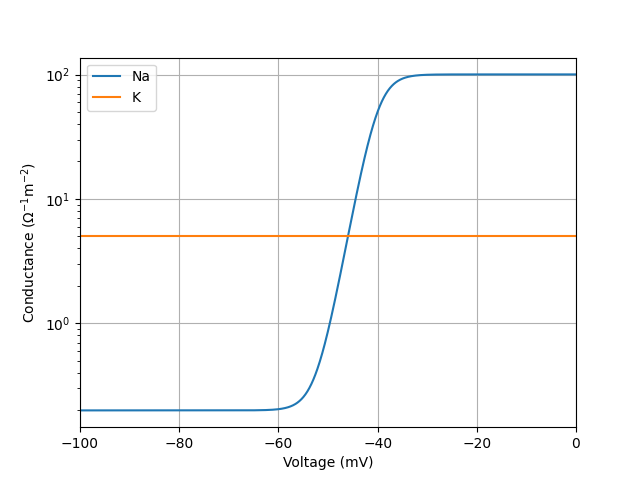
\includegraphics[width=10cm]{gNa.png}
  \caption{Na,Kチャネルのコンダクタンスの振る舞い}
  \label{fig:gNa}
\end{figure}

\begin{table}[htbp]
  \centering
  \caption{パラメータの意味とその値}
  \label{tab:params}
  \begin{tabular}{c|c|c}
    \hline
    パラメータ & 意味 & 値 \\
    \hline
    $\lambda$ & 電位が減衰するときの特徴的長さ(mm) &9.1\\
    $\tau$ & 電位が減衰するときの時定数(ms) &2\\
    $g_{K}$ & Kチャネルのコンダクタンス($\Omega^{-1}$m$^{-2}$) &5\\
    $V^{\mathrm{Na}}_{\mathrm{Nernst}}$ & Na$^{+}$のネルンスト電位(mV) &54\\
    $V^{\mathrm{K}}_{\mathrm{Nernst}}$ & K$^{+}$のネルンスト電位(mV) &$-75$\\
    $\beta q$ & Naチャネルのスイッチの急峻さ((mV)$^{-1}$) &0.5\\
    $V^{\ast}$ & Naチャネルのスイッチする電位(mV) &$-40$\\
    \hline
  \end{tabular}
\end{table}

\subsection{準備:シミュレーションの際の注意点}
シミュレーションの際は方程式\eqref{cable}を離散化して整理した式
\begin{equation}
  V_n(t+\Delta t) = V_n(t) + {\Delta t}\left[\frac{\lambda^2}{\tau} \frac{V_{n+1}(t) - 2V_n(t) + V_{n-1}(t)}{\Delta x^2} - \frac{f(V_n(t))}{\tau} \right] 
\end{equation}
を用いて計算を行う.
ただし$V(x,t)$を空間で離散化したものを$V_n(t)$と表記し,
\begin{equation}
  f(V_n(t)) = \frac{g_{\mathrm{Na}}(V_n(t))}{g_\mathrm{K}}(V_n(t)-V^{\mathrm{Na}}_{\mathrm{Nernst}}) + (V_n(t)-V^{\mathrm{K}}_{\mathrm{Nernst}}) 
\end{equation}
とした.
また$x=-50$\,mmから$x=50$\,mmの領域だけを考え,周期的境界条件を課す.

Pythonでシミュレーションを行う際,時間と位置の刻み幅に気をつける必要がある.
今回解く微分方程式\eqref{cable}は右辺を0とすれば拡散方程式となり,その拡散係数は
\begin{equation}
  D = \frac{\lambda^2}{\tau}
\end{equation}
となる.
この拡散方程式の数値計算が安定であるためには,時間の刻み幅$\Delta t$,位置の刻み幅$\Delta x$に対して
\begin{equation}
  \Delta x > \sqrt{2D\Delta t} \label{CFL}
\end{equation}
が成立する必要がある(Courant-Friedrichs-Lewy conditions).
この右辺が$\Delta t$の時間に拡散で移動する距離に対応することを考えると,直観的にはこの条件は「$\Delta t$時間経過しても$\Delta x$での電位の変化が微小に保たれるためには,$\Delta t$の間に拡散が$\Delta x$まで伝わってはならない」ということを表していると考えられる.
加えて,後で見るように今回の方程式の解に速さ
\begin{equation}
  v = \frac{\lambda}{\tau}
\end{equation}
で進行する波の解がある.
そのため同様に
\begin{equation}
  \Delta x > v\Delta t \label{vdt}
\end{equation}
も成立する必要がある.
ここで述べた式\eqref{CFL}および式\eqref{vdt}が成立するのは図\ref{fig:delta}の黄色の領域である.
今回はこの領域の範囲で,できるだけオレンジ色の境界からも離して刻み幅を選んだ.

\begin{figure}[htbp]
  \centering
  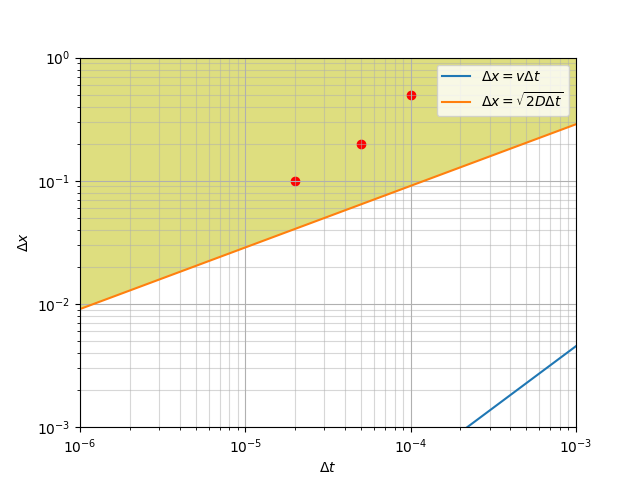
\includegraphics[width=10cm]{delta.png}
  \caption{数値解が安定となる刻み幅の領域(黄色)と今回用いた刻み幅(赤色)}
  \label{fig:delta}
\end{figure}

\subsection{問題:PBoC図17.19の再現}
表\ref{tab:params}に示したパラメータを代入して実際にケーブル方程式をPythonを用いてシミュレーションする.
具体的には初期条件として$x=0$を中心とする幅$\sigma=1$\,mm,下限$V_{mem}$,最大値$V_0$のガウス分布
\begin{equation}
  V(x,0) = (V_0 - V_{mem})\exp\left(-\frac{x^2}{\sigma^2} \right) + V_{mem}
\end{equation}
をとり,その時間発展を確認する.
このとき$V(x,t)$は常に偶関数なので,$x>0$の部分だけを図にする.

まず$V_0$の値を$-50$\,mVまたは$0$\,mVにとり,PBoCの図17.19を再現した(図\ref{fig:atte},図\ref{fig:wave}).
図\ref{fig:atte}より.$V_0$の値が小さいと周囲で脱分極が進行せず,信号が途絶えることが分かる.
一方図\ref{fig:wave}より,$V_0$の値が大きいと周囲でも脱分極が進行し,信号が伝搬することが分かる.
ただしPBoC表17.19のキャプションに「スナップショットは200\,ms間隔で示されている」とあるが,これは「200\,$\mu$s間隔」の誤りと考えられる\footnote{これは第2版でも修正されておらず,同じような誤植がPBoCの解答にも見つかった.}.

\begin{figure}[htbp]
  \centering
  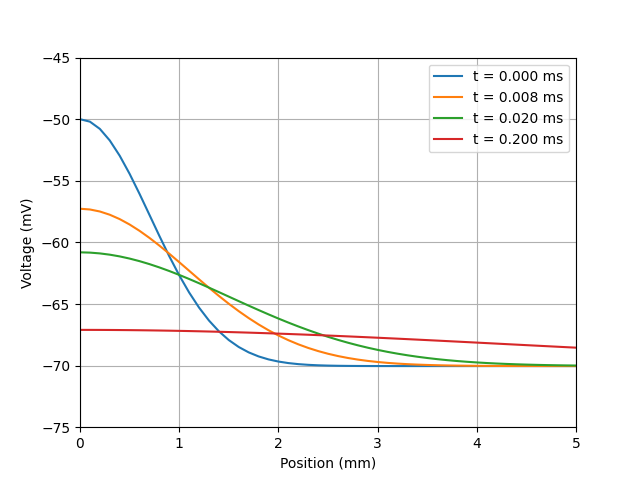
\includegraphics[width=10cm]{attenuation.png}
  \caption{PBoCの再現:最初の刺激が減衰していく様子($V_0=-50\,\mathrm{mV}$,$\Delta x=0.1$\,mm,$\Delta t = 2\times 10^{-5}$\,ms)}
  \label{fig:atte}
\end{figure}

\begin{figure}[htbp]
  \centering
  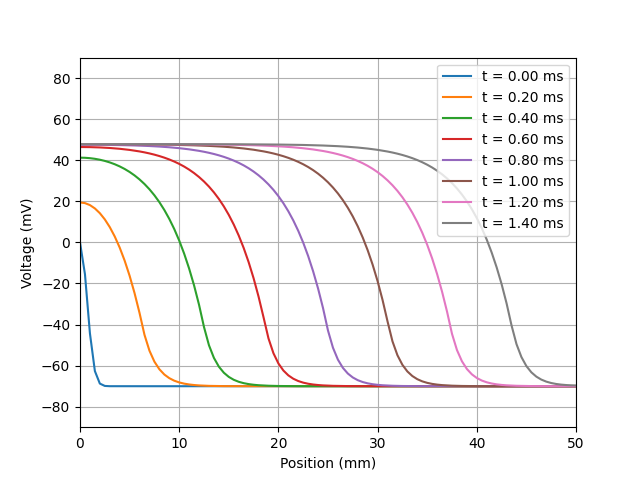
\includegraphics[width=10cm]{wave.png}
  \caption{PBoCの再現:波が伝播する様子($V_0=0\,\mathrm{mV}$,$\Delta x=0.5$\,mm,$\Delta t = 1\times 10^{-4}$\,ms)}
  \label{fig:wave}
\end{figure}

\subsection{補足:全か無かの法則}
また$V_0=0$\,mVの場合の解を詳しく見ると,最初の刺激が周囲に少し伝わった後,それによって周囲で脱分極が進行し,大きな波が形成される(図\ref{fig:attewave}).
加えて$V_0$を変えていくと,$V_0=-19$\,mVと$V_0=-20$\,mVで挙動が全く異なる(図\ref{fig:lim1},図\ref{fig:lim2}).
この結果から,$V_0$がある閾値を少しでも上回れば大きな信号が伝播し,閾値を少しでも下回れば信号が減衰することが分かる.
この現象は「全か無かの法則」と呼ばれる.
また初期条件として与えたガウス分布の幅$\sigma$を増やすと$V_0$の閾値が下がる(図\ref{fig:s_2}).
つまり$V_0$を増やすだけでなく$\sigma$を増やすことによっても伝搬する信号を作り出すことができる.

\begin{figure}[htbp]
  \centering
  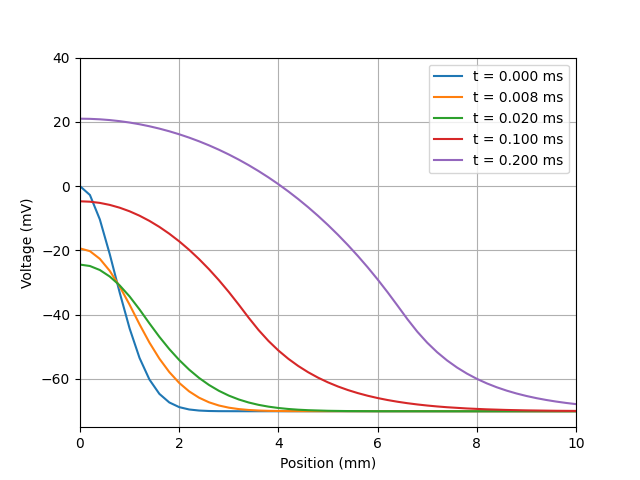
\includegraphics[width=10cm]{attewave.png}
  \caption{最初の刺激が一度拡散してから大きな波となる様子($V_0=0$\,mV,$\Delta x=0.2$\,mm,$\Delta t = 5\times 10^{-5}$\,ms))}
  \label{fig:attewave}
\end{figure}

\begin{figure}[htbp]
  \centering
  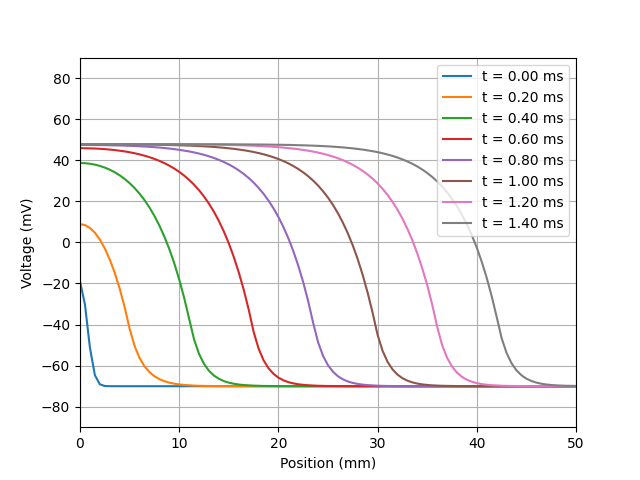
\includegraphics[width=10cm]{limit_-19mV.png}
  \caption{伝わるギリギリの信号が伝播する様子($V_0=-19$\,mV,$\Delta x=0.5$\,mm,$\Delta t = 1\times 10^{-4}$\,ms)}
  \label{fig:lim1}
\end{figure}

\begin{figure}[htbp]
  \centering
  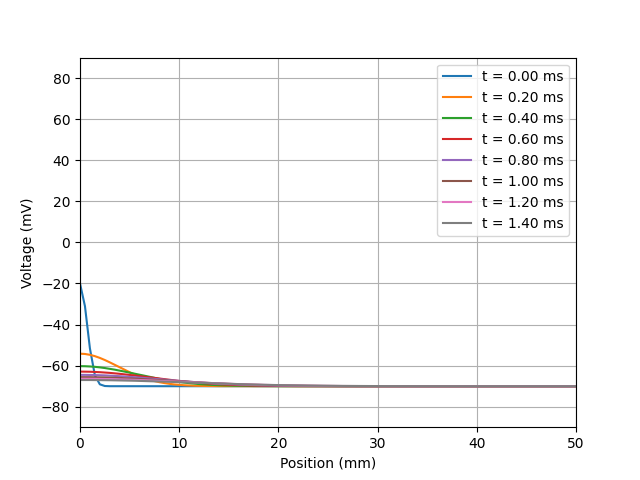
\includegraphics[width=10cm]{limit_-20mV.png}
  \caption{伝わらないギリギリの信号が減衰する様子($V_0=-20$\,mV,$\Delta x=0.5$\,mm,$\Delta t = 1\times 10^{-4}$\,ms)}
  \label{fig:lim2}
\end{figure}

\begin{figure}[htbp]
  \centering
  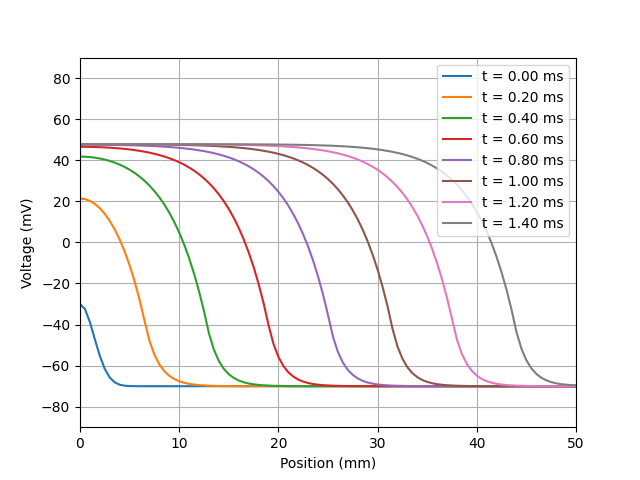
\includegraphics[width=10cm]{wave_s=2.png}
  \caption{閾値が下がる例.幅$\sigma=2$\,mmとした場合には$V_0=-30$\,mVでも信号が伝播した.($\Delta x=0.5$\,mm,$\Delta t = 1\times 10^{-4}$\,ms)}
  \label{fig:s_2}
\end{figure}

\section{補足:ホジキン-ハクスリー方程式}
問題17-6で議論したモデルは,一度ONになったNaチャネルはONのまま維持されていた.
ところが実際のニューロンではNaチャネルは一時的に開いた後2\,msのオーダーの時定数で再び閉じる.
つまりONになったNaチャネルは速やかに不活性化され,それによって波の背面で再びもとの分極が復活し,波はパルスの形になる.
このNaチャネルの不活性化に加えてKチャネルのコンダクタンスの変化も取り入れているモデルとして有名なものが,ホジキン-ハクスリーモデルである.
その詳細を述べる余裕はないが,ホジキン・ハクスリーの原論文(参考文献\cite{hh})通りのモデルをシミュレーションしたのでそれを添付する.
ただしこのシミュレーションは信号が軸索を伝播する効果(拡散項)は無視しており,1個の神経細胞に刺激を与える(定常電流を流す)状況を想定している.
$V$は膜電位(mV),$m_{\mathrm{K}}$はKチャネルが活性化している割合(0以上1以下),$I$は膜の外部から内部へ流れる単位面積あたりの電流($\mu$A/cm$^{2}$)である.
このシミュレーション結果から,外部から内部に大きな電流が流れると脱分極が起こり,Kチャネルの活性化によってもとの分極に戻ること(再分極),またその過程で膜電位が静止電位を下回ること(過分極)が読み取れる.

\begin{thebibliography}{99}
  \bibitem{srs}
    金子邦彦,澤井哲,高木拓明,古澤力「細胞の理論生物学 ダイナミクスの観点から」(2020)
  \bibitem{ghk}
    生理学研究所 基盤神経科学領域 神経シグナル研究部門 「分子神経情報学」講義資料(2006) \\
    \url{https://www.nips.ac.jp/huinfo/documents/lecture_06jan2006.pdf}
  \bibitem{ponp}
    Kanai, R., Ogawa, H., Vilsen, B. et al. Crystal structure of a Na$^+$-bound Na$^+$,K$^+$-ATPase preceding the E1P state. \textit{Nature} 502, 201–206 (2013). \\
    \url{https://doi.org/10.1038/nature12578} 
  \bibitem{select}
    一般社団法人 日本生物物理学会 イオン透過 \\
    \url{https://www.biophys.jp/highschool/C-03.html}
  \bibitem{hh}
    Hodgekin, A.L., and Huxley, A.F. 
    A quantitative description of membrane current and its application to conduction and excitation in nerve. 
    \textit{The Journal of Physiology.} 117(4): 500–544 (1952).
\end{thebibliography}

\end{document}